% try: change 24 to 36, or the 15 in rotate=15*\i: the rosette is drawn again as you type
\documentclass[tikz,border=0pt]{standalone}
\definecolor{navy}{HTML}{1D3E72}
\definecolor{c0}{HTML}{00A8A4}
\definecolor{c1}{HTML}{D3C72A}
\definecolor{c2}{HTML}{F0B225}
\definecolor{c3}{HTML}{F58F2D}

\begin{document}
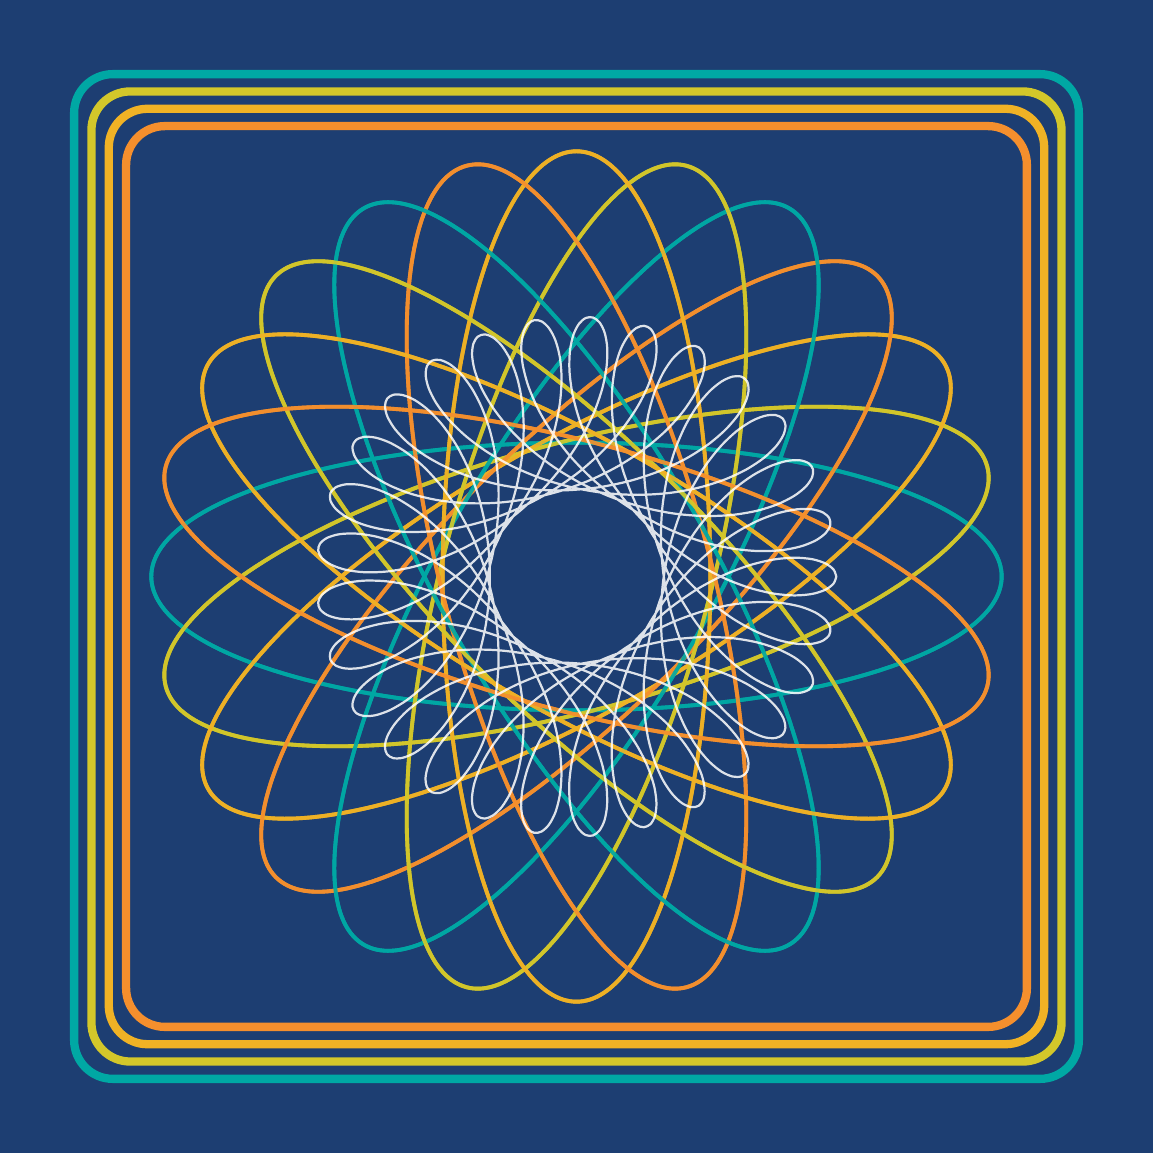
\begin{tikzpicture}
  \useasboundingbox (-6.97,-6.97) rectangle (6.97,6.97);
  \fill[navy] (-7.5,-7.5) rectangle (7.5,7.5);
  % a rosette of ellipses, the logo's four colours in turn
  \foreach \i in {0,...,23} {
    \pgfmathtruncatemacro\c{mod(\i,4)}
    \draw[line width=1.4pt, color=c\c, opacity=.9, rotate=15*\i] (0,0) ellipse (5.4cm and 1.7cm);
  }
  % a spirograph inside it
  \draw[line width=.8pt, white, opacity=.85, domain=0:6.2832*7, samples=600, smooth, variable=\t]
    plot ({2.2*cos(\t r) + 1.1*cos(2.2/0.7*\t r)}, {2.2*sin(\t r) - 1.1*sin(2.2/0.7*\t r)});
  % four stripes round the edge
  \foreach \c [count=\k] in {c0,c1,c2,c3}
    \draw[\c, line width=3pt, rounded corners=14pt] (-6.6+.22*\k,-6.6+.22*\k) rectangle (6.6-.22*\k,6.6-.22*\k);
\end{tikzpicture}
\end{document}
